\section{Versuch}

Es soll die molare Wärmekapazität bei konstantem Druck $C_p$ in Abhängigkeit der Temperatur gemessen werden.
Dazu wird eine Kupferprobe zunächst auf \SI{80}{\kelvin} abgekühlt.
Anschließend wird kontrolliert Energie zugeführt und sowohl die Energiemenge als auch der Temperaturanstieg gemessen.

\begin{figure}
	\centering
	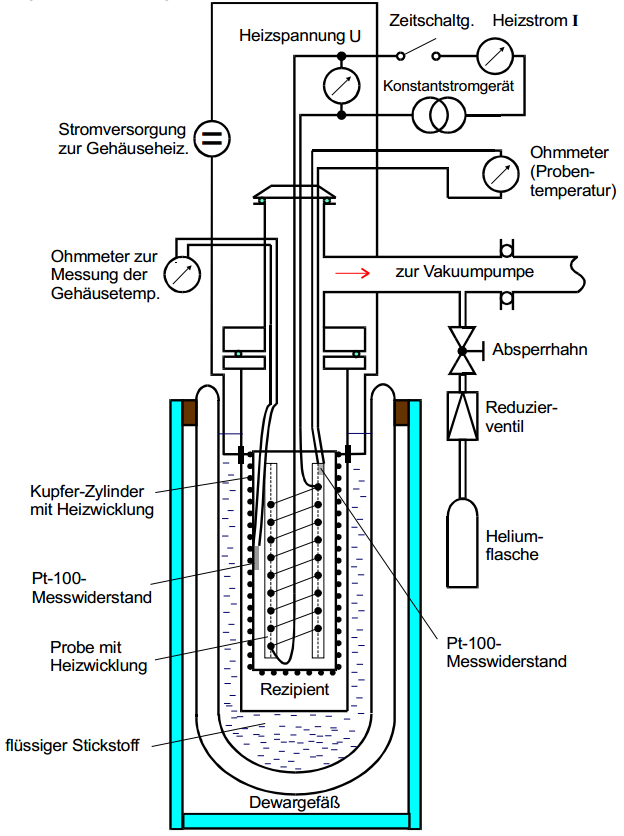
\includegraphics[width=0.8\textwidth]{img/aufbau.png}
	\caption{Schematischer Versuchsaufbau \cite{v47}}
	\label{fig:aufbau}
\end{figure}

Der Versuchsaufbau ist in Abbildung \ref{fig:aufbau} schematisch dargestellt.
Die Probe befindet sich in einem Rezipienten, der wiederum in einem Dewargefäß befestigt ist.
Zum Abkühlen der Probe wird flüssiger Stickstoff in das Dewargefäß gefüllt.
Während des Abkühlvorgangs wird der Rezipient mit Helium gefüllt, um den Wärmeübertrag von der Probe zum Stickstoff zu erleichtern.

Während der Messung wird die Probe mit einer Heizwicklung erhitzt.
Die angelegte Spannung und der Strom werden dabei aufgenommen, um die Heizleistung zu berechnen.
Zwei Pt-100-Messwiderstände sind an der Probe und am Rezipienten angebracht, mit denen die Temperaturen gemessen werden.

Es soll vermieden werden, dass mit der Probe, abgesehen von der kontrollierten Erwärmung, ein Wärmeaustausch stattfindet.
Um Wärmeübertragung durch Kontakt zu vermeiden, wird der Rezipient mit einer Vakuumpumpe evakuiert.
Weiterhin wird mit einer zweiten Heizwicklung der Rezipient erhitzt, sodass der Temperaturunterschied zwischen Rezipient und Probe möglichst gering ist.
So wird ein Wärmeaustausch durch Strahlung und durch das verbleibende Gas im Rezipienten vermieden.

Die Messung wird in Intervalle konstanter Heizleistung aufgeteilt, damit später einfach die zugeführte Energie für diese Zeiträume ausgerechnet werden kann.
Die Probe wird in Intervallen von $\SI{7}{\degree} - \SI{11}{\degree}$ erhitzt.
Zwischen den Intervallen wird ggf. der Heizstrom angepasst.